% A skeleton file for producing Computer Engineering reports
% https://kgcoe-git.rit.edu/jgm6496/KGCOEReport_template

\documentclass[CMPE]{../KGCOEReport}

% The following should be changed to represent your personal information
\newcommand{\classCode}{CMPE 460}  % 4 char code with number
\newcommand{\name}{Andrei Tumbar}
\newcommand{\LabSectionNum}{2}
\newcommand{\LabInstructor}{Beato}
\newcommand{\TAs}{Xavier Brooks\\
Diana Yakobchuk\\
Charles Poliwoda}
\newcommand{\LectureSectionNum}{1}
\newcommand{\LectureInstructor}{Beato}
\newcommand{\exerciseNumber}{8}
\newcommand{\exerciseDescription}{Heartbeat Monitor}
\newcommand{\dateDone}{April 1st}
\newcommand{\dateSubmitted}{April 17th}

\usepackage{tikz}
\usepackage{circuitikz}
\usetikzlibrary{calc}
\usetikzlibrary{circuits.logic.IEC,calc}
\usepackage{multirow}
\usepackage{float}
\usepackage{lmodern}
\usepackage{siunitx}
\usepackage{subcaption}
\usepackage{graphicx}
\usepackage[usestackEOL]{stackengine}
\usepackage{scalerel}
\usepackage[T1]{fontenc}
\usepackage{amsmath}
\usepackage{pdfpages}

\ctikzset{logic ports=ieee}

\def\lbar#1{\ThisStyle{%
    \setbox0=\hbox{$\SavedStyle#1$}%
    \stackengine{2.2\LMpt}{$\SavedStyle#1$}{\rule{\wd0}{0.1\LMpt}}{O}{c}{F}{F}{S}%
}}

\DeclareFontFamily{U}{mathx}{\hyphenchar\font45}
\DeclareFontShape{U}{mathx}{m}{n}{ <-> mathx10 }{}
\DeclareSymbolFont{mathx}{U}{mathx}{m}{n}
\DeclareFontSubstitution{U}{mathx}{m}{n}
\DeclareMathAccent{\widebar}{\mathalpha}{mathx}{"73}

\makeatletter
\newcommand{\cwidebar}[2][0]{{\mathpalette\@cwidebar{{#1}{#2}}}}
\newcommand{\@cwidebar}[2]{\@cwideb@r{#1}#2}
\newcommand{\@cwideb@r}[3]{%
    \sbox\z@{$\m@th\mkern-#2mu#3\mkern#2mu$}%
    \widebar{\box\z@}%
}
\newcommand\currentcoordinate{\the\tikz@lastxsaved,\the\tikz@lastysaved}
\makeatother

\newcommand\decbin[9]{%
    \par\smallskip
    \makebox[3cm][r]{$#1$\ }\fbox{#2}\,\fbox{#3}\,\fbox{#4}\,\fbox{#5}\,\fbox{#6}\,\fbox{#7}\,\fbox{#8}\,\fbox{#9}\par}


\def\code#1{\texttt{#1}}

\ctikzset{resistors/scale=0.8}

\ctikzset{logic ports/scale=0.7}

\begin{document}
    \maketitle
    \section*{Abstract}

    In this laboratory exercise a simple heartbeat monitor circuit was modeled and
    constructed on a breadboard. The purpose of the circuit was to filter a desired
    signal from a noisy circuit. Choosing the appropriate frequency ranges to filter
    out of an input signal with the goal of sending a measurable analog signal to the
    MSP432 microcontroller.

    \section*{Design Methodology}

	The heart rate monitor circuit is able to measure a low frequency periodic signal
	in the presence of noise. An optoisolator circuit is used to detect a heart beat
	in the neck or wrist. Small variations in the reflection of light against the
	OBP745 can be detected in the generated signal of the optoisolator.

	\begin{figure}[h!]
        \centering
        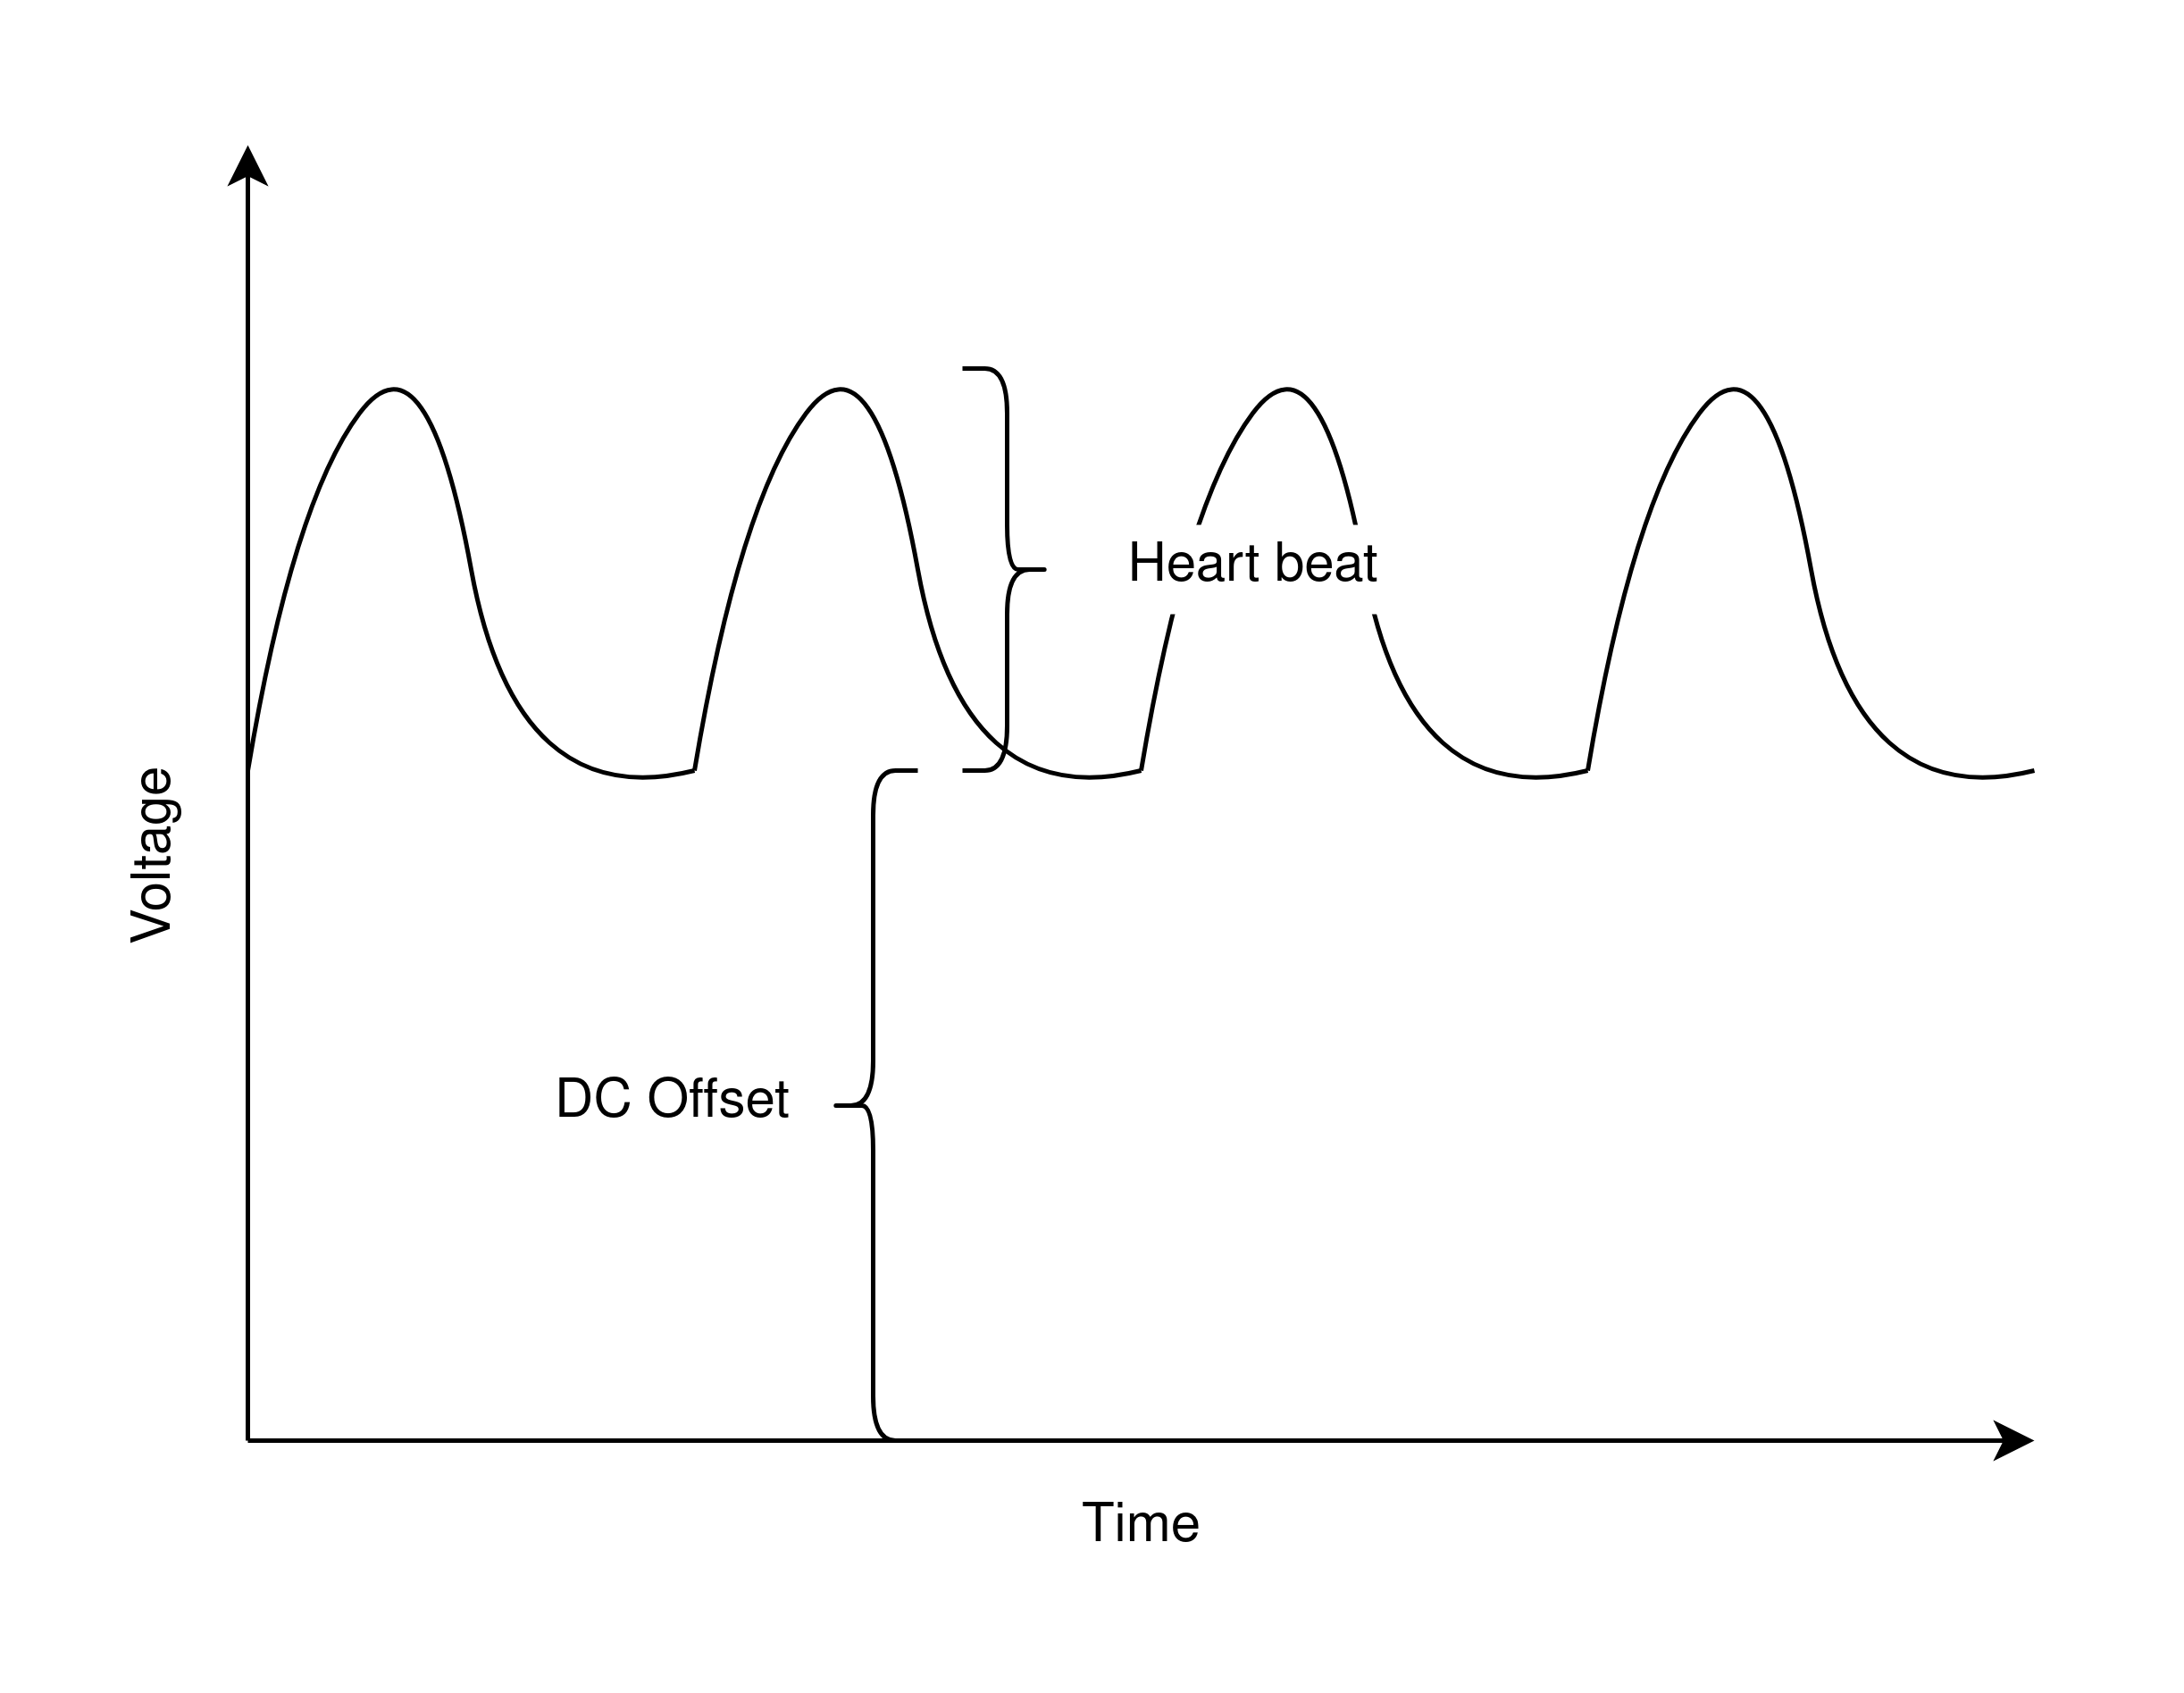
\includegraphics[width=12cm]{heartbeat}
        \caption{Example heartbeat signal from an optoisolator circuit.}
        \label{fig:heartbeat}
	\end{figure}

	Figure \ref{fig:heartbeat} shows an example of the signal generated by an optoisolator
	circuit if it were to be held up to the neck or wrist. Notice that the signal has a
	DC offset which comes from the fact that the heart beat signal will only vary the
	base voltage being output from the optoisolator. Figure \ref{fig:heartbeat} also
	does not show the noise from the optoisolator which would show up as higher frequency
	signals. High amount of noise will make the signal undetectable if it were directly
	fed into the microcontroller. Another challenge from the raw signal of the optoisolator
	is the amplitude of the wave itself. At an amplitude of about \SI{35}{\milli\volt},
	the signal is very difficult to detect on the microcontroller which accepts signals
	from \SI{0}{\volt} to \SI{3.3}{\volt}. \\

	All of these problems may be solved by filtering the signal generated by the
	optoisolator. The DC offset is in fact a \SI{0}{\hertz} signal and may be filtered
	out with a high-pass filter. The signal after a high pass filter with a relatively
	small cut-off frequency will look similar to the signal shown in Figure 
	\ref{fig:heartbeat}
	however it will not include the DC offset. The next issue is static noise. Static noise
	can be characterized as a signal with constant magnitude across all frequencies.
	Because our desired signal is of relatively low frequency when comparing the the
	frequency spectrum of static noise, the higher frequency noise will cause the signal
	to appear "fuzzy". To
	filter out this feature from the signal, a low-pass filter may be used. Choosing the
	correct cut-off frequencies for both the low-pass and the high-pass is key in
	designing the heartbeat monitor circuit.\\

	\subsection*{Low pass filter}
	While the average beats-per-minute of the heart may vary from person to person
	\cite{b1}, the maximum heart rate of humans is usually based on age. The older a
	person gets, the lower their maximum heartrate. At 20 years of age, the maximum
	heartrate is about 200 bpm \cite{b2}. While this number influences the cutoff
	frequency of the low-pass filter, 200 bpm (\SI{3.33}{\hertz}) should not be directly
	used as the cut off frequency. Firstly, the cut-off frequency is simply the
	\SI{-3}{\dB} point of the transfer function. This means that frequencies above this
	range will not be completely cut off. Another thing to consider is the fact that
	after the two filters, we must apply a voltage gain to scale the signal to a voltage
	range that is detectable by the microcontroller. Ideally, frequencies out of the
	range of the human heartbeat should not be amplified. For this reason, a lower
	frequency of \SI{2}{\hertz} was chosen as a low-pass cut-off frequency.\\

	\subsection*{High pass filter}
	The cutoff frequency of the high pass filter should be low enough to not cut
	off the desired signal, but also high enough to to properly filter out the DC offset.
	A frequency of \SI{0.5}{\hertz} was chosen.

	\pagebreak

	\subsection*{Schematic \& Simulation}

	As previously discussed, the heartbeat monitor circuit consists of a high-pass filter,
	followed by a low-pass filter, followed by a gain stage.

	\begin{figure}[h!]
        \centering
        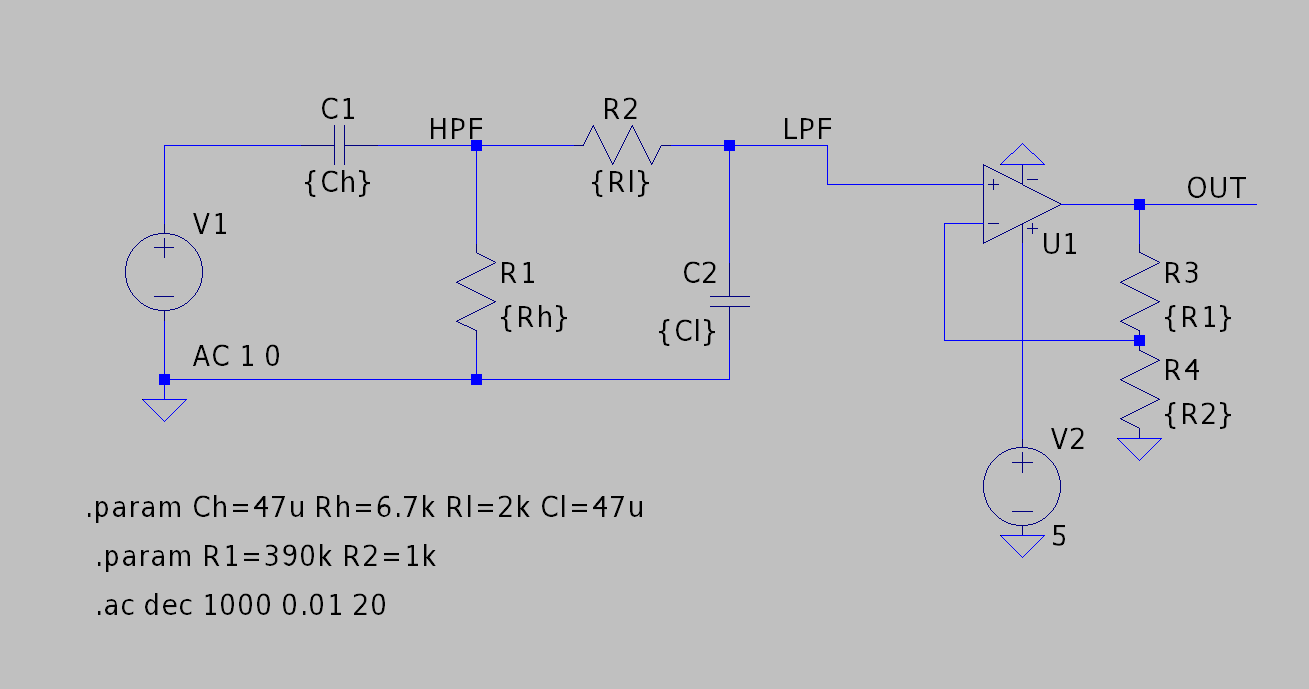
\includegraphics[width=12cm]{schematic}
        \caption{Schematic layout of heartbeat monitor.}
        \label{fig:schematic}
	\end{figure}

	As seen in Figure \ref{fig:schematic}, the values chosen for the resistors and
	capacitors in high and low pass filters will yield cutoff frequencies of
	\SI{.505}{\hertz} and \SI{1.693}{\hertz} respectively.
	These numbers are slightly off from the chosen cutoff frequencies due to resistor
	availability limitations in the lab. Finally the gain stage is meant boost the
	gain of the filtered optoisolator signal from \SI{35}{\milli\volt} to about
	\SI{3}{\volt}. Looking at the schematic, 

    \section*{Results}

	

    \section*{Conclusion}

	\section*{Questions}

	\begin{enumerate}
	\item
	IRQ flags need to be cleared in the interrupt service routine because otherwise
	the CPU could immediately interrupt again and essentially be forever block inside
	the interrupt.
	\item
	Different interrupts will run different ISRs. For example, there is a unique ISR for
	each switch on the board. If the peripheral uses the same ISR for multiple pins,
	a unique flag will be set in one of the status or IRQ registers on the peripheral.  
	\item
	The initiation of the the camera data transfer happens in four distinct steps
	running at \SI{200}{\kilo\Hz}:
	\begin{enumerate}
	\item \code{SI} goes high,
	      \code{CLK} stays low
	\item \code{SI} stays high,
		  \code{CLK} goes high
	\item \code{SI} goes low,
		  \code{CLK} stays high
	\item \code{SI} stays low,
		  \code{CLK} goes low
	\end{enumerate}
	\end{enumerate}

	\begin{thebibliography}{00}
\bibitem{b1} F. Arvin, S. Doraisamy, and E. Safar Khorasani, “Frequency shifting approach towards textual transcription of Heartbeat sounds,” Biological procedures online, 04-Oct-2011. [Online]. Available: https://www.ncbi.nlm.nih.gov/pmc/articles/PMC3396354/. [Accessed: 16-Apr-2022].
\bibitem{b2} B. Gholipour, “What is a normal heart rate?,” LiveScience, 13-Dec-2021. [Online]. Available: https://www.livescience.com/42081-normal-heart-rate.html. [Accessed: 16-Apr-2022].
	\end{thebibliography}

\end{document}